\documentclass{article}
\usepackage[T1]{fontenc}
\usepackage[utf8]{inputenc}
\usepackage{amsmath}
\usepackage{amssymb}
\usepackage{hyperref}
\usepackage{parskip} %skip the indent of a new paragraph.
\usepackage{float}
\usepackage{graphicx}
\usepackage{listings}
\usepackage[export]{adjustbox}
\usepackage{tabstackengine}
\usepackage{color}
\lstset{language=Matlab, frame=single, breaklines=true,numbers=left, keywordstyle=\color{blue},rulecolor=\color{black},commentstyle=\color{gray}}

\usepackage{cleveref}
\usepackage{todonotes}

\renewcommand{\vec}[1]{\mathbf{#1}}
%\newcommand{\TODO}[1]{\todo[inline]{#1}}


\title{Linear Systems TTK4115 - Helicopter Assignement}
\author{-- 759494 -- \\  -- 748434 -- }
\date{\today}%September 2016 TODO}

\begin{document}

\begin{titlepage}
    \maketitle
    \rule{\linewidth}{0.5mm}
    
    %\begin{abstract}
    %Lorem testum testater testtest. Test.
    %\end{abstract}
    
    \begin{figure}
    \centering
    
\includegraphics[width=0.5\textwidth]{logontnu_eng}
    \end{figure}
    \thispagestyle{empty}
\end{titlepage}

%\section*{Table of contents} 
\tableofcontents
\thispagestyle{empty} %Avoid page numbering on the table of contents
\newpage    


\setcounter{page}{1}
\section{Mathematical Modeling}

\subsection{Equations of Motion}
The equations of motion for the pitch, travel- and elevation angle were derived on the basis of Newton's second law for rotation:
%
\begin{equation}
    \sum \vec{\tau}_{z} = \sum \vec{r}_i\times\vec{F}_i = \sum(\vec{m_i}\vec{r_i^2})\vec{\alpha}_z= J\alpha_z \label{EOR}
\end{equation}
%

%
Where $\vec{\tau}$ is the torque about the given axis (z), $\alpha$ is the angular acceleration and $J$ is the moment of inertia around the given point, given a rigid body and that the cross-product is defined \cite{uniphysics}.
In our assignement we used the illustrations shown in \cref{fig:illustrasjon} as a basis for our mathematical models.\\ Also given were the relations between the forces and voltages and equations for the moments of inertia for each joint:
%
\begin{subequations}
    \begin{align}
    F_f &= K_fV_f   \nonumber              \\
    F_b &= K_fV_b   \nonumber               \\ \nonumber \\
    J_p &= 2m_pl_p^2                           \label{eq:MOI1} \\
    J_e &= m_cl_c^2 + 2m_pl_h^2                \label{eq_MOI2}\\
    J_\lambda &= m_cl_c^2 + 2m_p(l_h^2+l_p^2)  \label{eq:MOI3}  %\tag{2c}
    \end{align}
\end{subequations}
%
\begin{figure}[b]
    \centering
    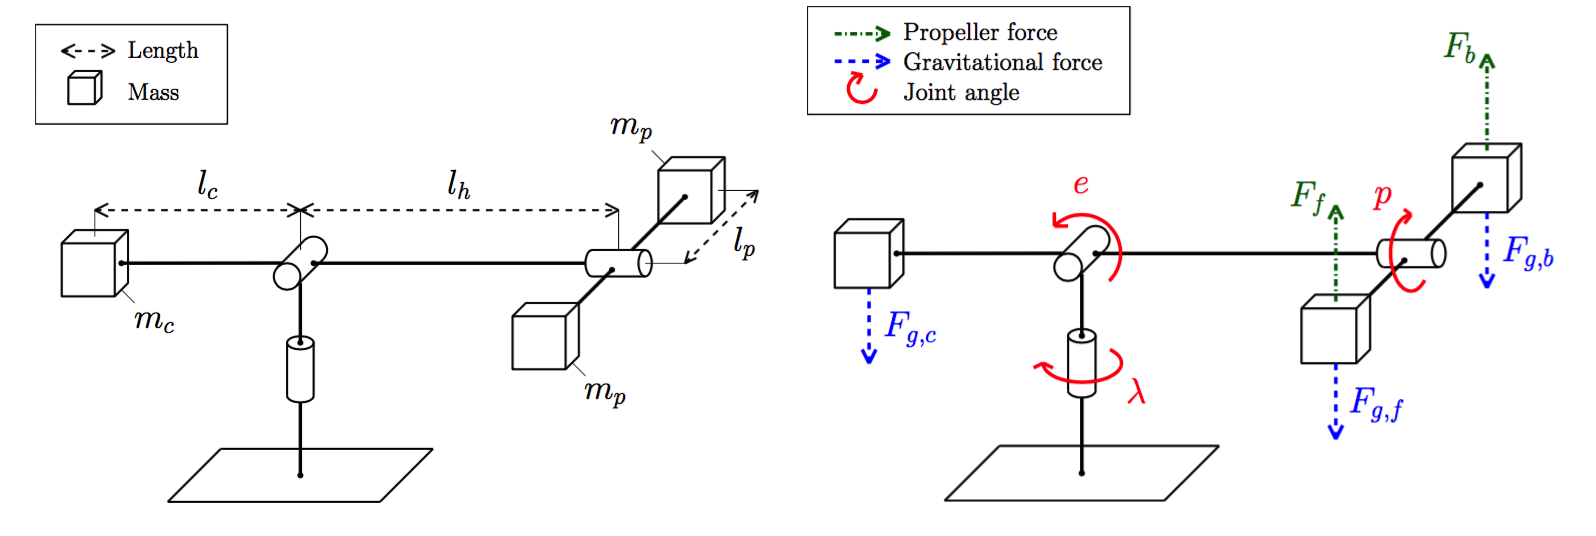
\includegraphics[width=1.0\textwidth]{helikopter.png}
    \caption{Illustration and free body diagram of our helicopter model. Image credit: \cite{labtext}}
    \label{fig:illustrasjon}
\end{figure}
Here $p$ is the pitch angle, $e$ is the elevation angle, $\lambda$ is the travel angle and $J_x$ is the respective moment of intertia.

%%%%%%%%%%%%%%%%%%%%%%%%%%%%%%%%%%%%%%%%%%%%%%%%%%%%%%%%%%%%%%%%%%%%%%

\subsubsection*{Pitch (p) :}
\begin{align*}
    \sum\vec{\tau_p} &= l_p(F_f-F_b) + l_p\cos(p)(F_{g,p}-F_{g,f})\\
     &= l_pK_f(V_f-V_b) 
\end{align*}
Then using Newton's 2nd. law of rotation (eq.\ref{EOR}):
\begin{equation}
    J_p\ddot{p} = l_pK_fV_d = L_1V_d \tag{3a}\label{3a}
\end{equation}

%%%%%%%%%%%%%%%%%%%%%%%%%%%%%%%%%%%%%%%%%%%%%%%%%%%%%%%%%%%%%%%%%%%%%%

\subsubsection*{Elevation (e) :}
\begin{align*}
    \sum\vec{\tau} &= l_h(F_f+F_b) + [-l_h(F_{g,f}+F_{g,b})]\cos(e) + l_cF_{g,c}\cos(e)\\
    &= l_hK_fV_s\cos(p) + g\cos(e)(l_cm_c - 2l_hm_p)
\end{align*}
Then from (eq.\ref{EOR}):
\begin{equation}
    J_e\ddot{e} = L_3V_s\cos(p) + L_2\cos(e) \tag{3b} \label{3b}
\end{equation}

%%%%%%%%%%%%%%%%%%%%%%%%%%%%%%%%%%%%%%%%%%%%%%%%%%%%%%%%%%%%%%%%%%%%%%

\subsubsection*{Travel ($\lambda$) :}
\begin{align*}
    \sum\vec{\tau} &= -l_h(F_f+F_b)\sin(p)\cos(e)\\
    &= -l_hK_fV_s\sin(p)\cos(e)
\end{align*}
Which again leaves us with
\begin{equation}
    J_\lambda\ddot{\lambda} = L_4V_s\sin(p)\cos(e) \tag{3c}\label{3c}
\end{equation}


%%%%%%%%%%%%%%%%%%%%%%%%%%%%%%%%%%%%%%%%%%%%%%%%%%%%%%%%%%%%%%%%%%%%%%
\newpage %??
\subsection{Linearization}
We want to linearize the system around the given point of equilibrium $(p, e, \lambda)^T$ = $[p^*, e^*, \lambda^*]^T = (0, 0, 0)^T \quad \forall t \quad\Rightarrow\quad [\ddot{p},\ddot{e},\ddot{\lambda}]^T = (0,0,0)^T$. Inserting  \cref{3a}-(\ref{3c}) into $(V_s,V_c)^T = (V_s^{*},V_d^{*})^T$ gives us
%
\begin{align*}
    V_{s,e}^* = -\frac{L_2}{L_3}&\frac{\cos(e)}{\cos(p)} = -\frac{L_2}{L_3}\\
    V_{s,\lambda}^* &= 0\\
    0 = l_pK_fV_d^* \quad &\Rightarrow\quad V_d^* = 0\\
    \Rightarrow\begin{bmatrix}V_s^* \\ V_d^*\end{bmatrix} &= \begin{bmatrix}-\frac{L_2}{L_3}\\0\end{bmatrix} 
\end{align*}
%
We now introduce the coordinate transformation
\setcounter{equation}{3}
%
\begin{align*}
    \begin{bmatrix}\widetilde{p}\\\widetilde{e}\\\widetilde{\lambda} \end{bmatrix}
    = \begin{bmatrix}p\\e\\\lambda\end{bmatrix}
    - \begin{bmatrix}p^*\\e^*\\\lambda^*\end{bmatrix}
    \quad\text{and}\quad
    \begin{bmatrix}\tilde{V_s}\\\tilde{V_d} \end{bmatrix}
    = \begin{bmatrix}V_s\\V_d\end{bmatrix}
    - \begin{bmatrix}V_s^*\\V_d^*\end{bmatrix}  %\tag{4}
\end{align*}
%
The equations \ref{3a} - \ref{3c} then transform into
%
\setcounter{equation}{3}
\begin{align}
    \begin{bmatrix}\widetilde{p}\\\widetilde{e}\\\widetilde{\lambda} \end{bmatrix}
    = \begin{bmatrix}\frac{L_1}{J_p}(\tilde{V_d}+V_d^*) - p^*  \\ 
    \frac{L_2}{J_e}\cos(\widetilde e + e^*)+\frac{L_3}{J_e}(\tilde{V_s}+V_s^*)\cos(\widetilde{p}+p^*) - e^*  \\  
    \frac{L_4}{J_\lambda}(\tilde{V_s}+V_s^*)\cos(\widetilde{e}+e^*)\sin(\widetilde{p}+p^*) - \lambda^*  \end{bmatrix} %\tag{5}
\end{align}
%
Defining the states and input as $\vec{x} = [\widetilde{p},\widetilde{e},\widetilde{\lambda}]^T$ and $\vec{u} = [\tilde{V_s},\tilde{V_d}]^T$ giving $\vec{h} = \vec{h}(\vec{x},\vec{u}) = [\ddot{\widetilde{p}},\ddot{\widetilde{e}},\ddot{\widetilde{\lambda}}]^T$ around the equilibrium point $(x_0,u_0)$. The transformed system can them be written in a state-space form \cite{chen2014linear}:
%
\begin{align*}
    \vec{\widetilde{x}} = \vec{A}\vec{x} + \vec{B}\vec{u}
\end{align*}
%
where 
%
\begin{align*}
    \vec{A} = \frac{\partial\vec{h}}{\partial\vec{x}}\bigg|_{(x_0,u_0)}
    \quad\text{and}\quad
    \vec{B} = \frac{\partial\vec{h}}{\partial\vec{u}}\bigg|_{(x_0,u_0)}
\end{align*} 
%
This results in the state-space model
%
\begin{align}
    \vec{\ddot{x}} = 
    \begin{bmatrix}0&0&0\\0&0&0\\\frac{L_4}{J_\lambda}&0&0
    \end{bmatrix}
    \vec{x} + 
    \begin{bmatrix}0&\frac{L_1}{J_p}\\\frac{L_3}{J_3}&0\\0&0
    \end{bmatrix}
    \vec{u} %\tag{6}\label{eq.6}
\end{align}
%
Which corresponds to
\begin{subequations}
\begin{align}
    \ddot{\widetilde{p}} &= \frac{L_1}{J_p}\tilde{V_d} = K_1\tilde{V_d}   \\%\tag{7a}\\
    \ddot{\widetilde{e}} &= \frac{L_3}{J_e}\tilde{V_s} = K_2\tilde{V_s}   \\%\tag{7b}\\
    \ddot{\widetilde{\lambda}} &= \frac{L_4}{J_\lambda}\tilde{V_s^*}\widetilde{p} = K_3\widetilde{p} \label{eq:6c}
\end{align}
\end{subequations}

%%%%%%%%%%%%%%%%%%%%%%%%%%%%%%%%%%%%%%%%%%%%%%%%%%%%%%%%%%%%%%%%%%%%%%
\subsection{Physical Behaviour Around Equilibrium}

Since linearization of non-linear systems only provide an approximation of the model in question, it is valid mostly around the defined operating point (equilibrium), but breaks if one deviates too far. This holds for feedforward and other types of linearized controllers. We had a hard time controlling the helicopter using just feedforward control, possibly slightly better performance around the equilibrium, but difficult to notice. The helicopter was also seemingly eager to oscillate given small pitch adjustments. 

%%%%%%%%%%%%%%%%%%%%%%%%%%%%%%%%%%%%%%%%%%%%%%%%%%%%%%%%%%%%%%%%%%%%%%

\subsection{Determining the Motor Force Constant}
The motor force constant $K_f$ was determined by firstly measuring the the voltage $V_s = V_s^*$ which kept the helicopter at equilibrium $(e = e^* = 0)$. $V_s$ was measured to be $7.2 $ V. The values for $e$ and $V_s$ was then inserted into (\ref{3b}) resulting in 
%
\begin{align*}
    K_f = -g\dfrac{l_cm_c-2l_hm_p}{V_sl_h} = \underline{0.1387}.
\end{align*}
%
This value is used in the following problems.


\section{Monovariable Control}


\subsection{PD Controller}
Given the controller
\begin{align}
    \tilde{V_d} = K_{pp}(\widetilde{p}_c-\widetilde{p}) - K_{pd}\dot{\tilde{p}} 
    \quad\quad, K_{pp},K{pd} >0  \label{PDcont}
\end{align}
with reference pitch $\widetilde{p}_c$. To find the transfer function $\frac{\tilde{p}}{\tilde{p}_c}(s)$ we insert (\ref{PDcont}) into (6a) and then laplace transform:
%
\begin{align}
    \ddot{\tilde{p}} &= K_1K_{pp}(\tilde{p}_c-\tilde{p}) - K_1K_{pd}\dot{\tilde{p}}\nonumber\\
    s^2\tilde{p} &= K_1K_{pp}\tilde{p}_c - K_1K_{pp}\tilde{p} - K_1K_{pd}s\tilde{p}\nonumber\\
    \Rightarrow \dfrac{\tilde{p}}{\tilde{p}_c}(s) &= \frac{K_1K_{pp}}{s^2+K_1K_{pd}+K_1K_{pp}}  \label{transf}
\end{align}
%
Comparing this transfer function to a standard 2nd. order transfer function
%
\begin{align*}
    h(s) = \frac{1}{(\frac{s}{\omega_0})^2 + 2\zeta\frac{s}{\omega_0} + 1}
\end{align*}
%
we get the following equations for $K_{pp}$ and $K_{pd}$ which we based our actual values on:
%
\begin{align}
    \omega_0 &= \sqrt{K_1K_{pp}}                     \nonumber\\
    \frac{\zeta}{\omega_0} &= \frac{K_{pd}}{2K_{pp}} \nonumber\\
    K_{pd} &= 2\frac{\sqrt{K_1K_{pp}}}{K_1}          \label{Kpd}
\end{align}
%
This is under the condition that $\zeta = 1$, giving a critically damped system.


%%%%%%%%%%%%%%%%%%%%%%%%%%%%%%%%%%%%%%%%%%%%%%%%%%%%%%%%%%%


\section{Multivariable Control}

Using the system described by (6a)-(6b) we get the following state-space model
\begin{equation}
    \vec{\dot{x}} = \begin{bmatrix}     % A
                                0&1&0\\
                                0&0&0\\
                                0&0&0
                    \end{bmatrix}
                    \begin{bmatrix}     % x
                                \tilde{p}\\
                                \dot{\tilde{p}}\\
                                \tilde{e}
                    \end{bmatrix}
                    +
                    \begin{bmatrix}     % B
                                0&0\\
                                0&K_1\\
                                K_2&0
                    \end{bmatrix}
                    \begin{bmatrix}     % u
                                \tilde{V_s}\\
                                \tilde{V_d}
                    \end{bmatrix}
\end{equation}
%
\subsection{Controllability and LQR}
The controllability matrix for a $3\times3$ system is given by
\begin{equation}
    \begin{bmatrix}
            B & AB & A^2B
    \end{bmatrix}
    =
    \begin{bmatrix}
            0&0&0&K_1&0&0\\
            0&K_1&0&0&0&0\\
            K_2&0&0&0&0&0
    \end{bmatrix}
\end{equation}
which has $ rank = n = 3 $. Thus the system is controllable.\\ \\
Now we will use a controller on the form $$ \vec{u} = \vec{Pr}-\vec{Kx}$$
where the input $\vec{u} = -\vec{Kx}$ minimizes the costfunction 
$$J = \int_{0}^{\infty}(\vec{x}^T(t)\vec{Qx}(t) + \vec{u}^T(t)\vec{Ru}(t))dt $$ and $\vec{r} = [\tilde{p}_c \quad \dot{\tilde{e}}_c]^T$. $\vec{K}$ here corresponds to the linear quadratic regulator and $\vec{Q}$ and $\vec{R}$ are diagonal matrices. \\

The matrix $\vec{P}$ is found such that $\lim_{t\rightarrow\infty}\tilde{p}=\tilde{p}_c$ and $\lim_{t\rightarrow\infty}\dot{\tilde{e}} = \dot{\tilde{e}}_c$:
\begin{align}
    \dot{\vec{x}} &= \vec{Ax} + \vec{Bu}    \nonumber\\ \nonumber
    &= \vec{Ax} + \vec{B(Pr-Kx)} = 0\\\nonumber
    \Rightarrow& (\vec{A}-\vec{BK})\vec{x}_\infty = -\vec{BP}\vec{r}_0\\\nonumber
    \Rightarrow& \vec{y}_\infty = [\vec{C}(\vec{BK}-\vec{A})^{-1}\vec{B}]\vec{Pr}_0 \nonumber\\ \nonumber\\
    \text{which in turn gives}\nonumber\\ \nonumber\\
    \vec{P} &= [\vec{C}(\vec{BK}-\vec{A})^{-1}\vec{B}]^{-1} \label{Pmatrix}
\end{align}



Our weighting matrices were as follows
%
\begin{align*}
    \vec{Q} = \begin{bmatrix}
                15&0&0\\
                0&1&0\\
                0&0&10
            \end{bmatrix} 
    \quad
    \vec{R} = \begin{bmatrix}
                0.1&0\\
                0&0.3
            \end{bmatrix}
\end{align*}
%
The elements of the matrix $\vec{Q}$ were chosen such that it penalized deviations in the pitch and elevation rate, i.e. $\vec{Q}_{11}$ and $\vec{Q}_{33}$ were increased. $\vec{Q}_{11} < \vec{Q}_{33}$ gave less elevation control from the helicopter, thus we chose $\vec{Q}_{11} > \vec{Q}_{33}$ as shown. \\
The elements of R were set a bit lower as to "lower the cost" of using input. $\vec{R}_{22}$ were chosen larger than $\vec{R}_{11}$ as the opposite gave o.k. control, but resulted in a trade-off in regard to elevation vs pitch control. \\

The resulting $\vec{K}$ matrix were found using the MATLAB-command 
%
\begin{lstlisting}  
    K = lqr(A, B, Q, R);
\end{lstlisting}
%
then the $\vec{P}$ matrix were calculated using \cref{Pmatrix}, giving
%
\begin{align*}
    \vec{K} =   \begin{bmatrix}
                    0       & 0      & 10 \\
                    7.07    & 5.12   & 0
                 \end{bmatrix}
        \quad \quad
    \vec{P} =   \begin{bmatrix}
                    0       & 10 \\
                    7.07    & 0
                \end{bmatrix} .
\end{align*}
%
%
%
%\newpage
\subsection{LQR with PI}

To include a PI-controller in our model we introduce two new states 
$$  \dot{\gamma} = \tilde{p} - \tilde{p}_c $$ 
$$  \dot{\zeta} = \tilde{e} - \tilde{e}_c  $$
which gives a new state vector 
$\vec{x} = [\tilde{p} \enskip \dot{\tilde{p}} \enskip \dot{\tilde{e}} \enskip \gamma \enskip \zeta]^T$. This in turn gives the new state-space matrices
\begin{align*}
    \vec{A} =   \begin{bmatrix}
                    0&1&0&0&0&0\\
                    0&0&0&0&0&0\\
                    0&0&0&0&0&0\\
                    1&0&0&0&0&0\\
                    0&0&1&0&0&0
                \end{bmatrix}
        \quad
    \vec{B} =   \begin{bmatrix}
                    0&0\\
                    0&K_1\\
                    K_2&0\\
                    0&0\\
                    0&0
                \end{bmatrix}
\end{align*}
as well as a new $\vec{Q}$ matrix 
$$\vec{Q} = \begin{bmatrix}
                15&0&0&0&0\\
                0&1&0&0&0\\
                0&0&10&0&0\\
                0&0&0&2&0\\
                0&0&0&0&10
            \end{bmatrix}.
$$
This state expansion also increases the dimensions of $\vec{K}$, which is calculated as before. $\vec{P}$ can't now be calculated as before, but observing that 
$$
\vec{K} =   \begin{bmatrix}
                \vec{K}{11} & ... & \vec{K}_{1m}\\
                .&.&.\\
                .&.&.\\
                .&.&.\\
                \vec{K}_{n1} & ... & \vec{K}_{nm}
            \end{bmatrix}
    \quad \Rightarrow \quad
\vec{P} =   \begin{bmatrix}
                \vec{K}_{11} & \vec{K}_{1m}\\
                \vec{K}_{n1} & \vec{K}_{nm}
            \end{bmatrix}
$$
throughout, simplifies the calculations for $\vec{P}$.\\
The PI controller performed better overall than the P controller. With the PI we were able to get faster to steady-state without overshooting as well as getting proper elevation control with constant input.
\section{State Estimation}
\subsection{Estimation State-matrices}

%% State Space Model
Using equation (6a-6c) we derived the following matrices for the state space model

% $$
%     \ddot{\widetilde{p}} = K_1 \tilde{V_d} %\xrightarrow{\int}K_1 \tilde{V_d} t %\xrightarrow{\int} \frac{1}{2} K_1 %\tilde{V_d} t^2 = \widetilde{p}
% $$

% $$
%     \ddot{\widetilde{e}} = K_2 %\tilde{V_s}\xrightarrow{\int}K_2 \tilde{V_s} %t\xrightarrow{\int} \frac{1}{2} K_1 %\widetilde{V_s} t^2 = \widetilde{e}
% $$
% $
% \ddot{\widetilde{\lambda}} = K_3 %\widetilde{p}\xrightarrow{\int}K_3 %\widetilde{p} t\xrightarrow{\int} \frac{1}{2} %K_3 \widetilde{p} t^2 = \widetilde{e}
% $$

\begin{align}
    A = \begin{bmatrix}0&1&0&0&0&0\\0&0&0&0&0&0\\0&0&0&1&0&0\\0&0&0&0&0&0\\0&0&0&0&0&1\\ K_3&0&0&0&0&0 \end{bmatrix} 
    \quad   
    B = \begin{bmatrix} 0&0\\0&K_1\\0&0\\K_2&0\\0&0\\0&0 \end{bmatrix} 
    \quad 
    C = \begin{bmatrix} 1&0&0&0&0&0 \\ 0&0&1&0&0&0 \\ 0&0&0&0&1&0 \end{bmatrix}
\end{align}

with state vectors

\begin{align}
    x = \begin{bmatrix}
        \tilde{p}\\
        \dot{\tilde{p}}\\
        \tilde{e}\\
        \dot{\widetilde{e}}\\
        \tilde{\lambda}\\
        \dot{\tilde{\lambda}} 
        \end{bmatrix}, \quad
    u = \begin{bmatrix}
        \tilde{V_s}\\
        \tilde{V_d} 
        \end{bmatrix}, \quad
    y = \begin{bmatrix}    
        \tilde{p}\\
        \tilde{e}\\
        \tilde{\lambda} 
        \end{bmatrix}
\end{align}


%%Observability Mat

\subsection{Observability and State Observer}
In order to examine the state observer we calculated the observability matrix, which is given by
\begin{equation*}
    \mathcal{O} = 
    %\fixTABheight{}
    \bracketMatrixstack{
        C\\CA\\\vdots{}\\CA^5    
    }
\end{equation*}

which has $ rank = n = 6 $, thus the system is observable.\\
The linear observer used is given by
%
\begin{equation*}
    \dot{\vec{x}} = \vec{A\hat{x}} + \vec{Bu} + \vec{L}(\vec{Y} - \vec{C\hat{x}})
\end{equation*}
%
where $\vec{L}$ is the observer gain matrix. 
To calculate $\vec{L}$ we first looked at the eigenvalues of our system $(\vec{A}-\vec{BK})$, then adjusting the poles such that the estimator becomes 10-100 faster. $\vec{L}$ was calculated by using the MATLAB-command
%
\begin{lstlisting}  
    L = place(A', B', poles)';
\end{lstlisting}
%
The poles were placed on a circle with radius 40 in the complex plane (\cref{fig:poles}). This resulted in fast control without the noise affecting the system too much. Choosing a smaller radius made the estimator too slow, while increasing the radius too much led to a very noisy signal, as shown in figure \cref{fig:plot1} and \cref{fig:plot2}


\begin{figure}[H]
    \centering
    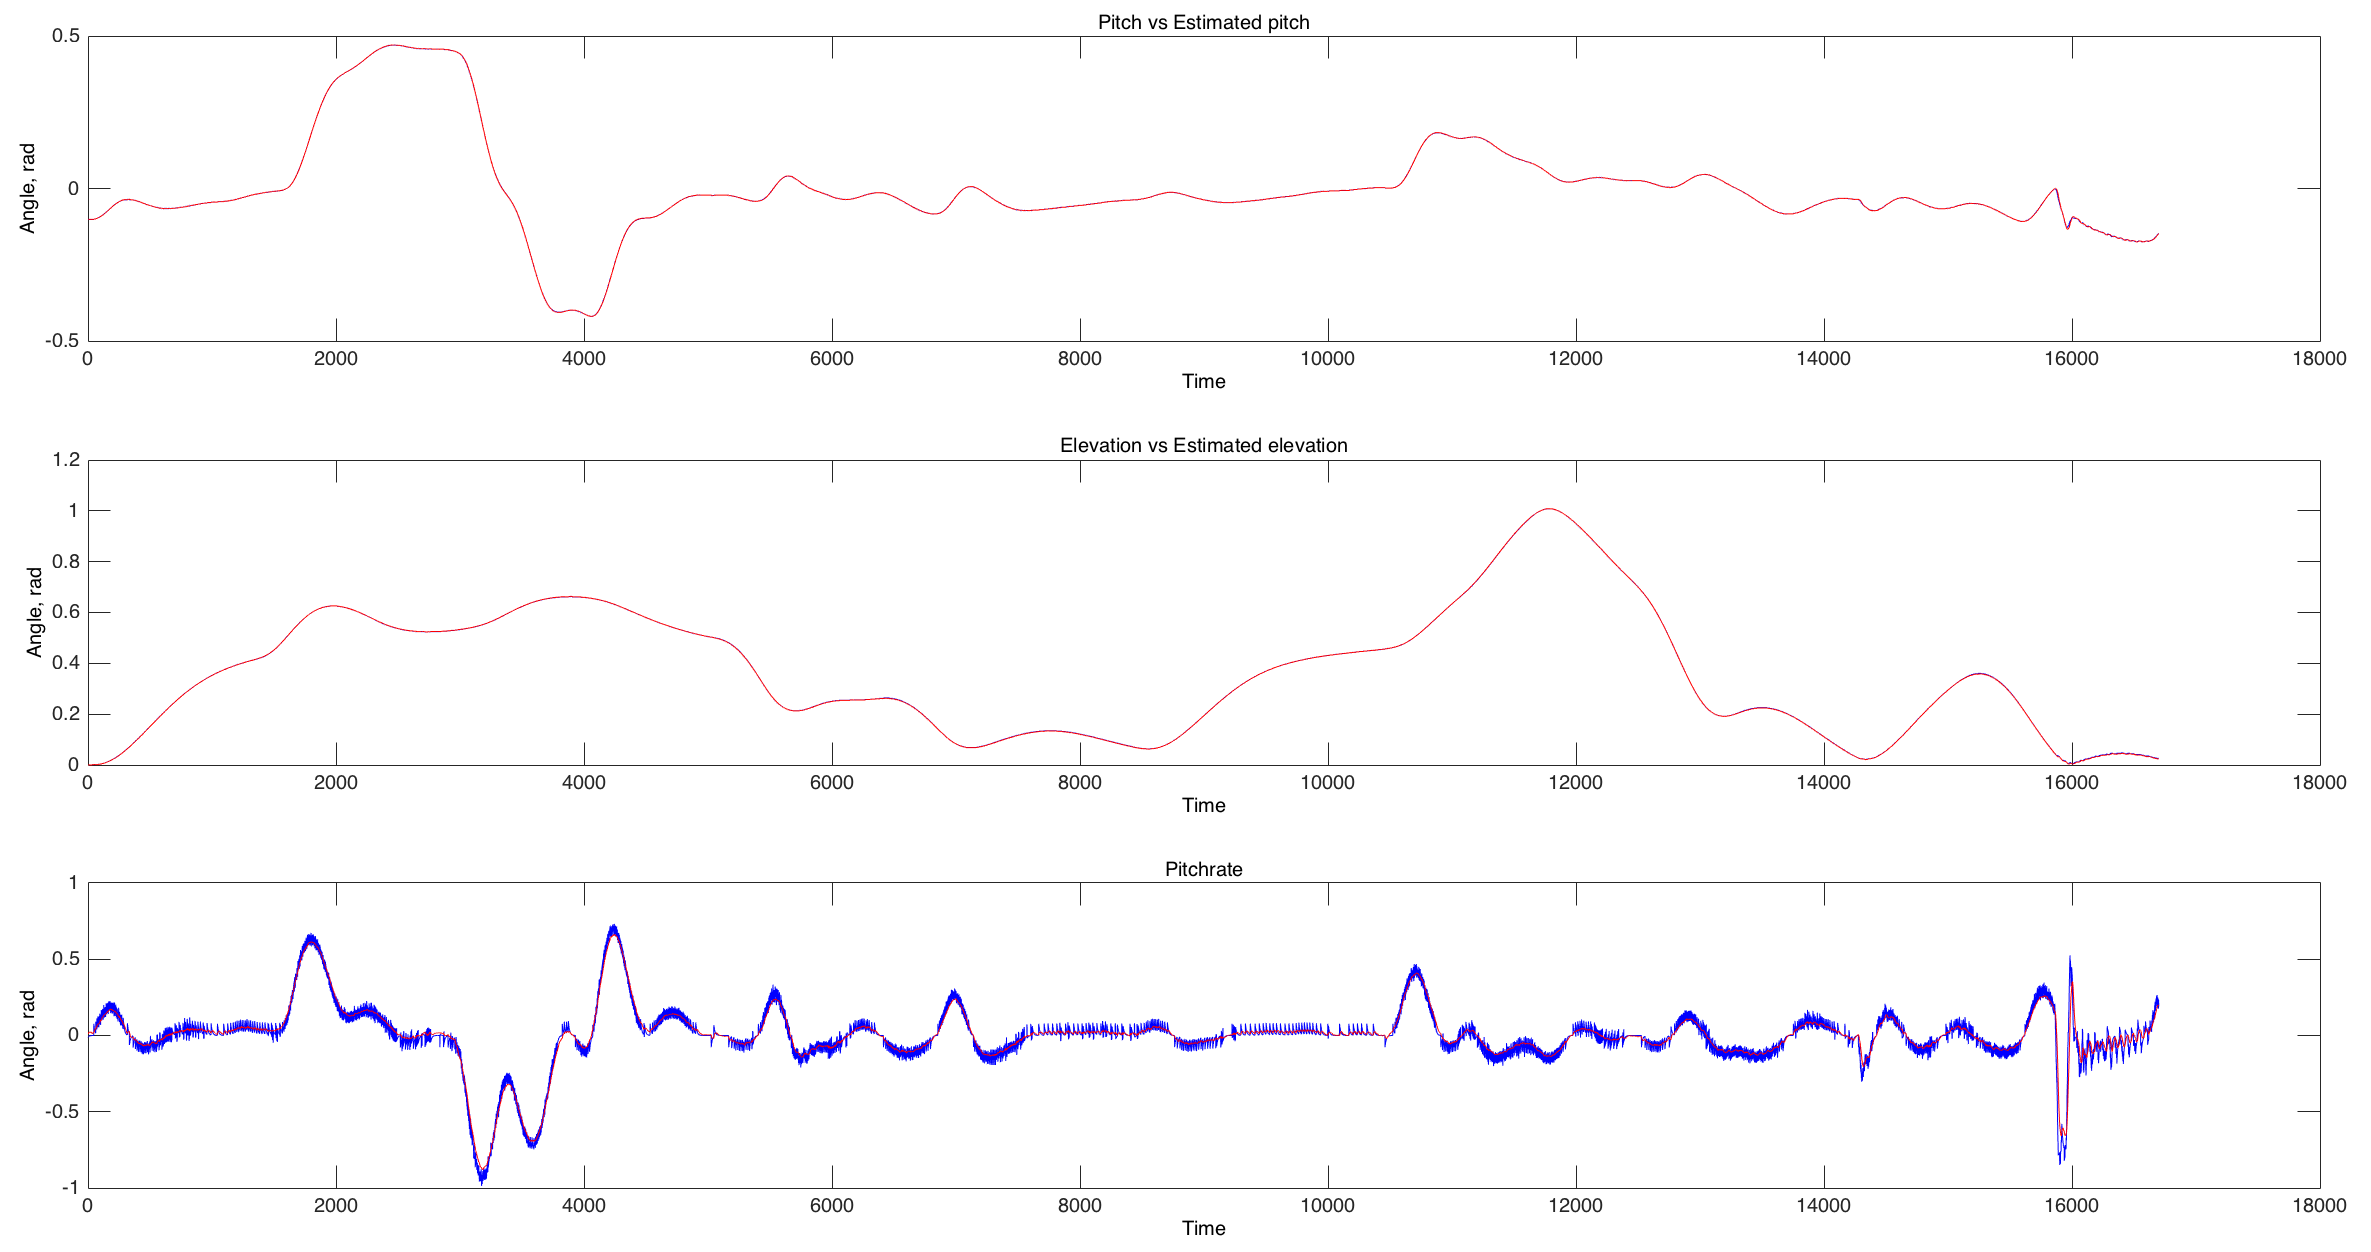
\includegraphics[width=1.0\textwidth]{pitchNpitchrate_P.png}
    \caption{Comparison of measured and estimated values of pitch, elevation and pitch rate in the P-controller (\emph{\color{blue}Blue} = measured value, \emph{\color{red} red} = estimated value)}
    \label{fig:plot1}
\end{figure}

\begin{figure}[H]
    \centering
    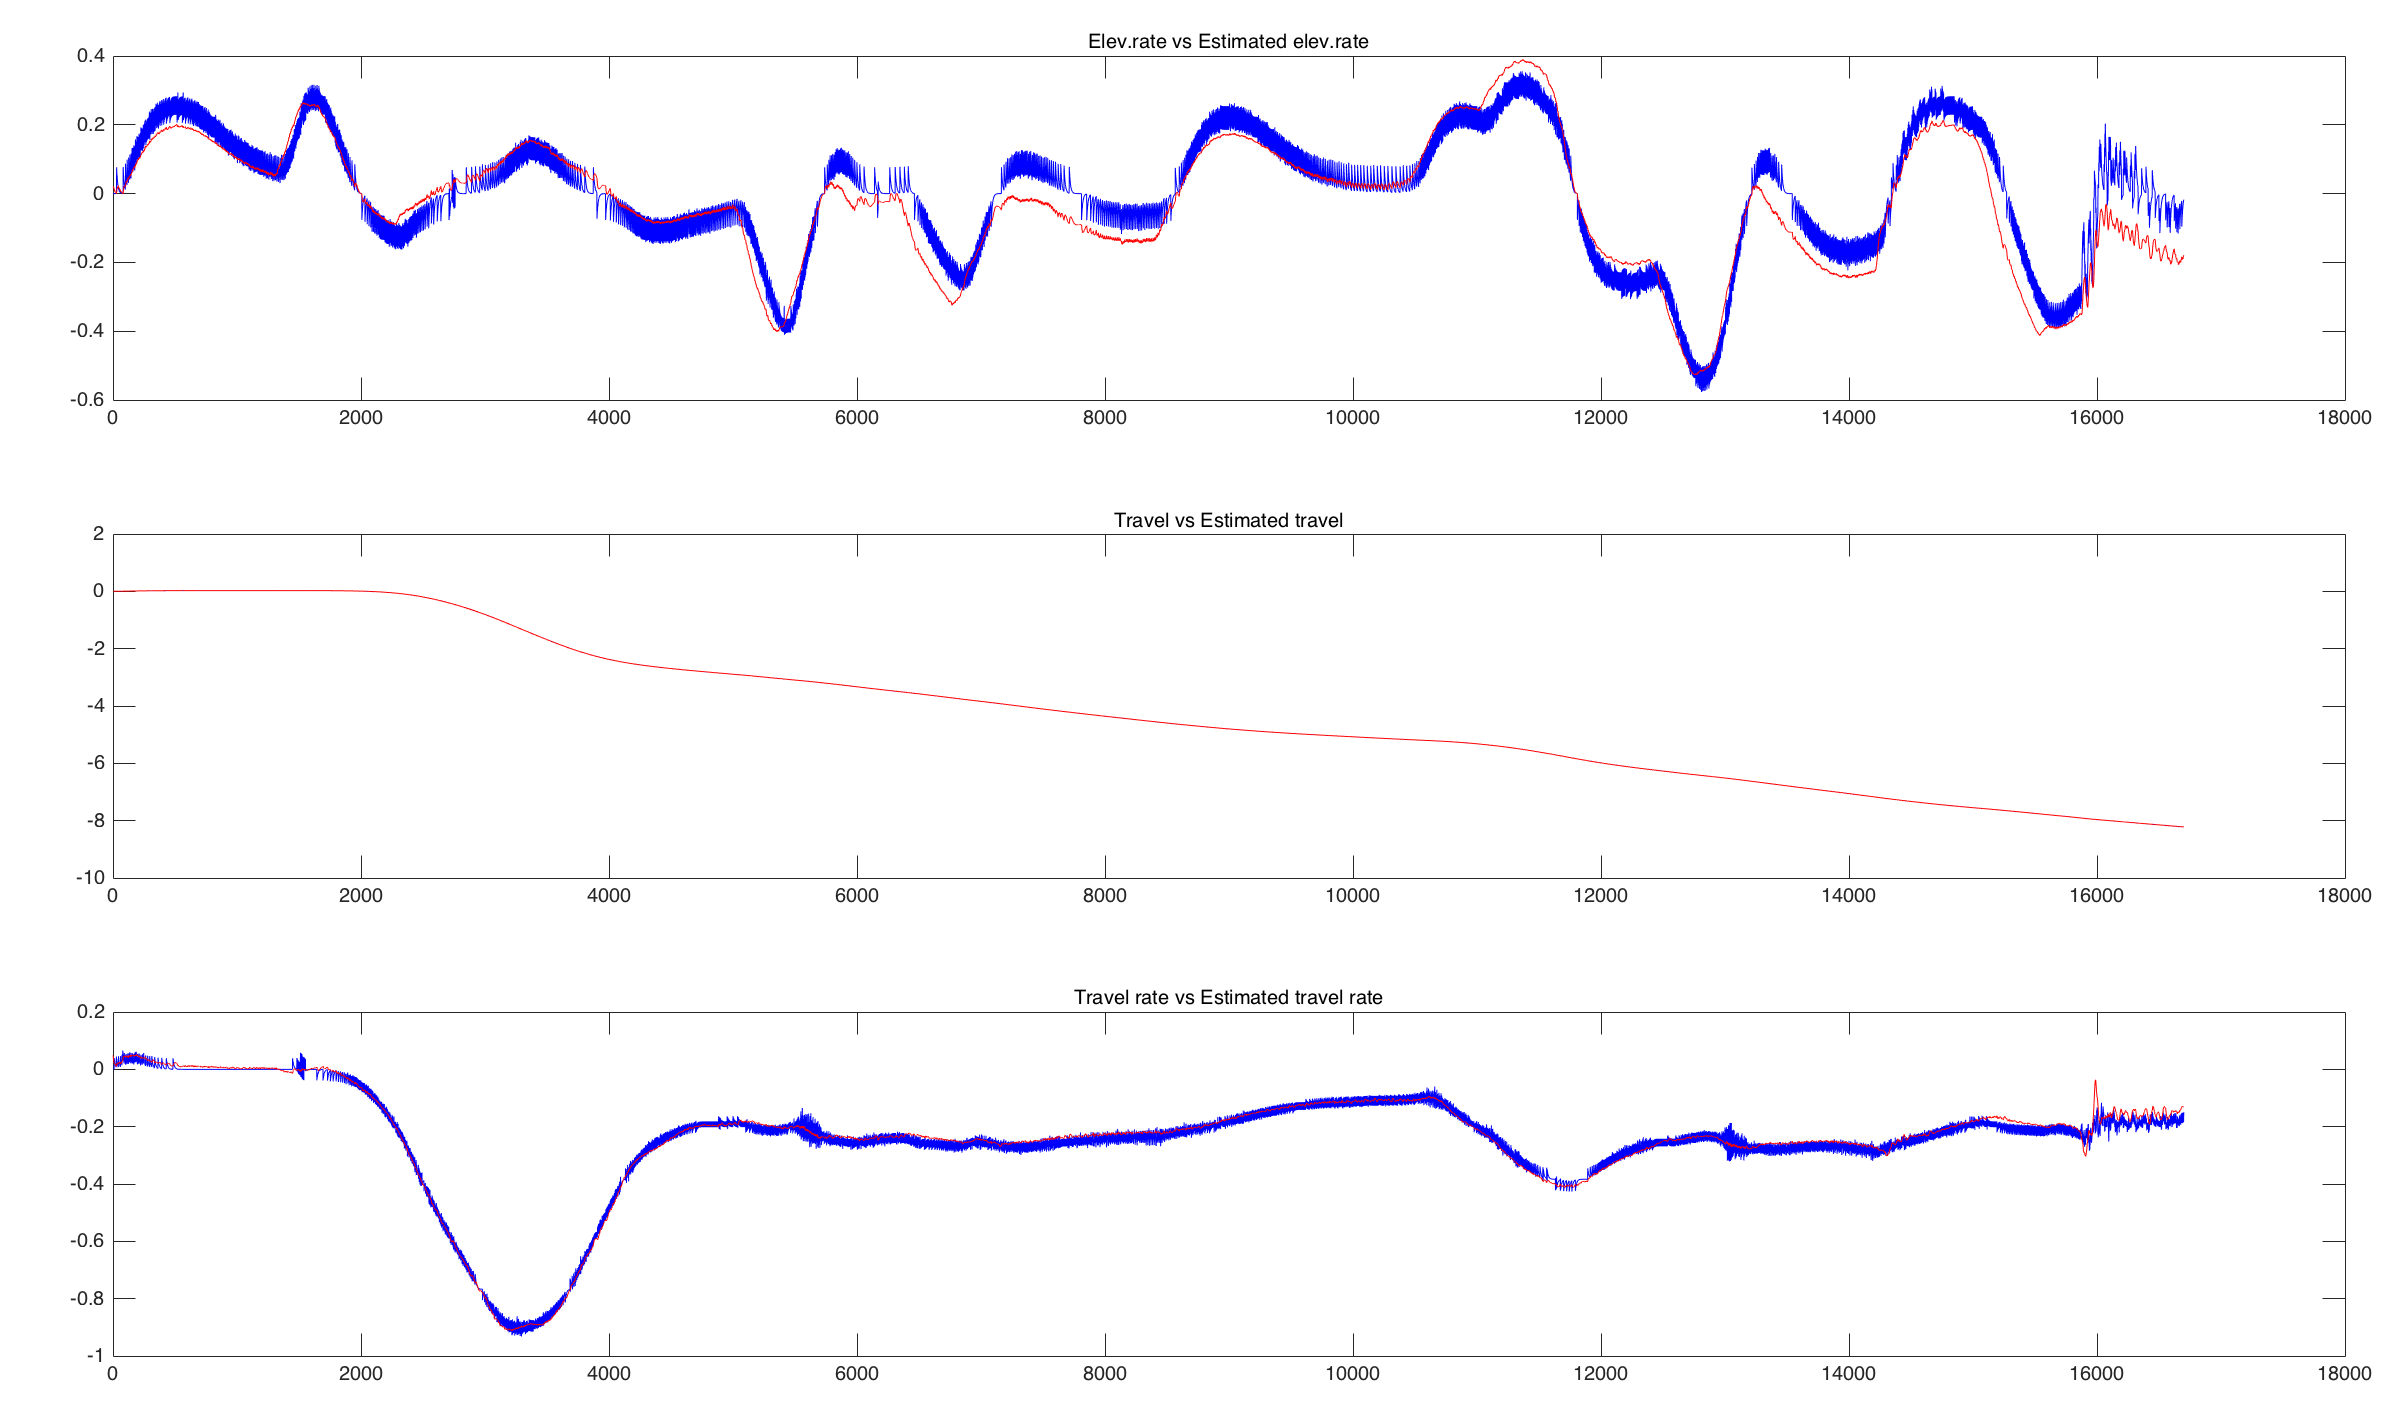
\includegraphics[width=1.0\textwidth]{elevrateP.png}
    \caption{Comparison of measured and estimated values of elevation rate, travel and travel rate in the P-controller (\emph{\color{blue}Blue} = measured value, \emph{\color{red} red} = estimated value)}
    \label{fig:plot2}
\end{figure}

\begin{figure}[H]
    \centering
    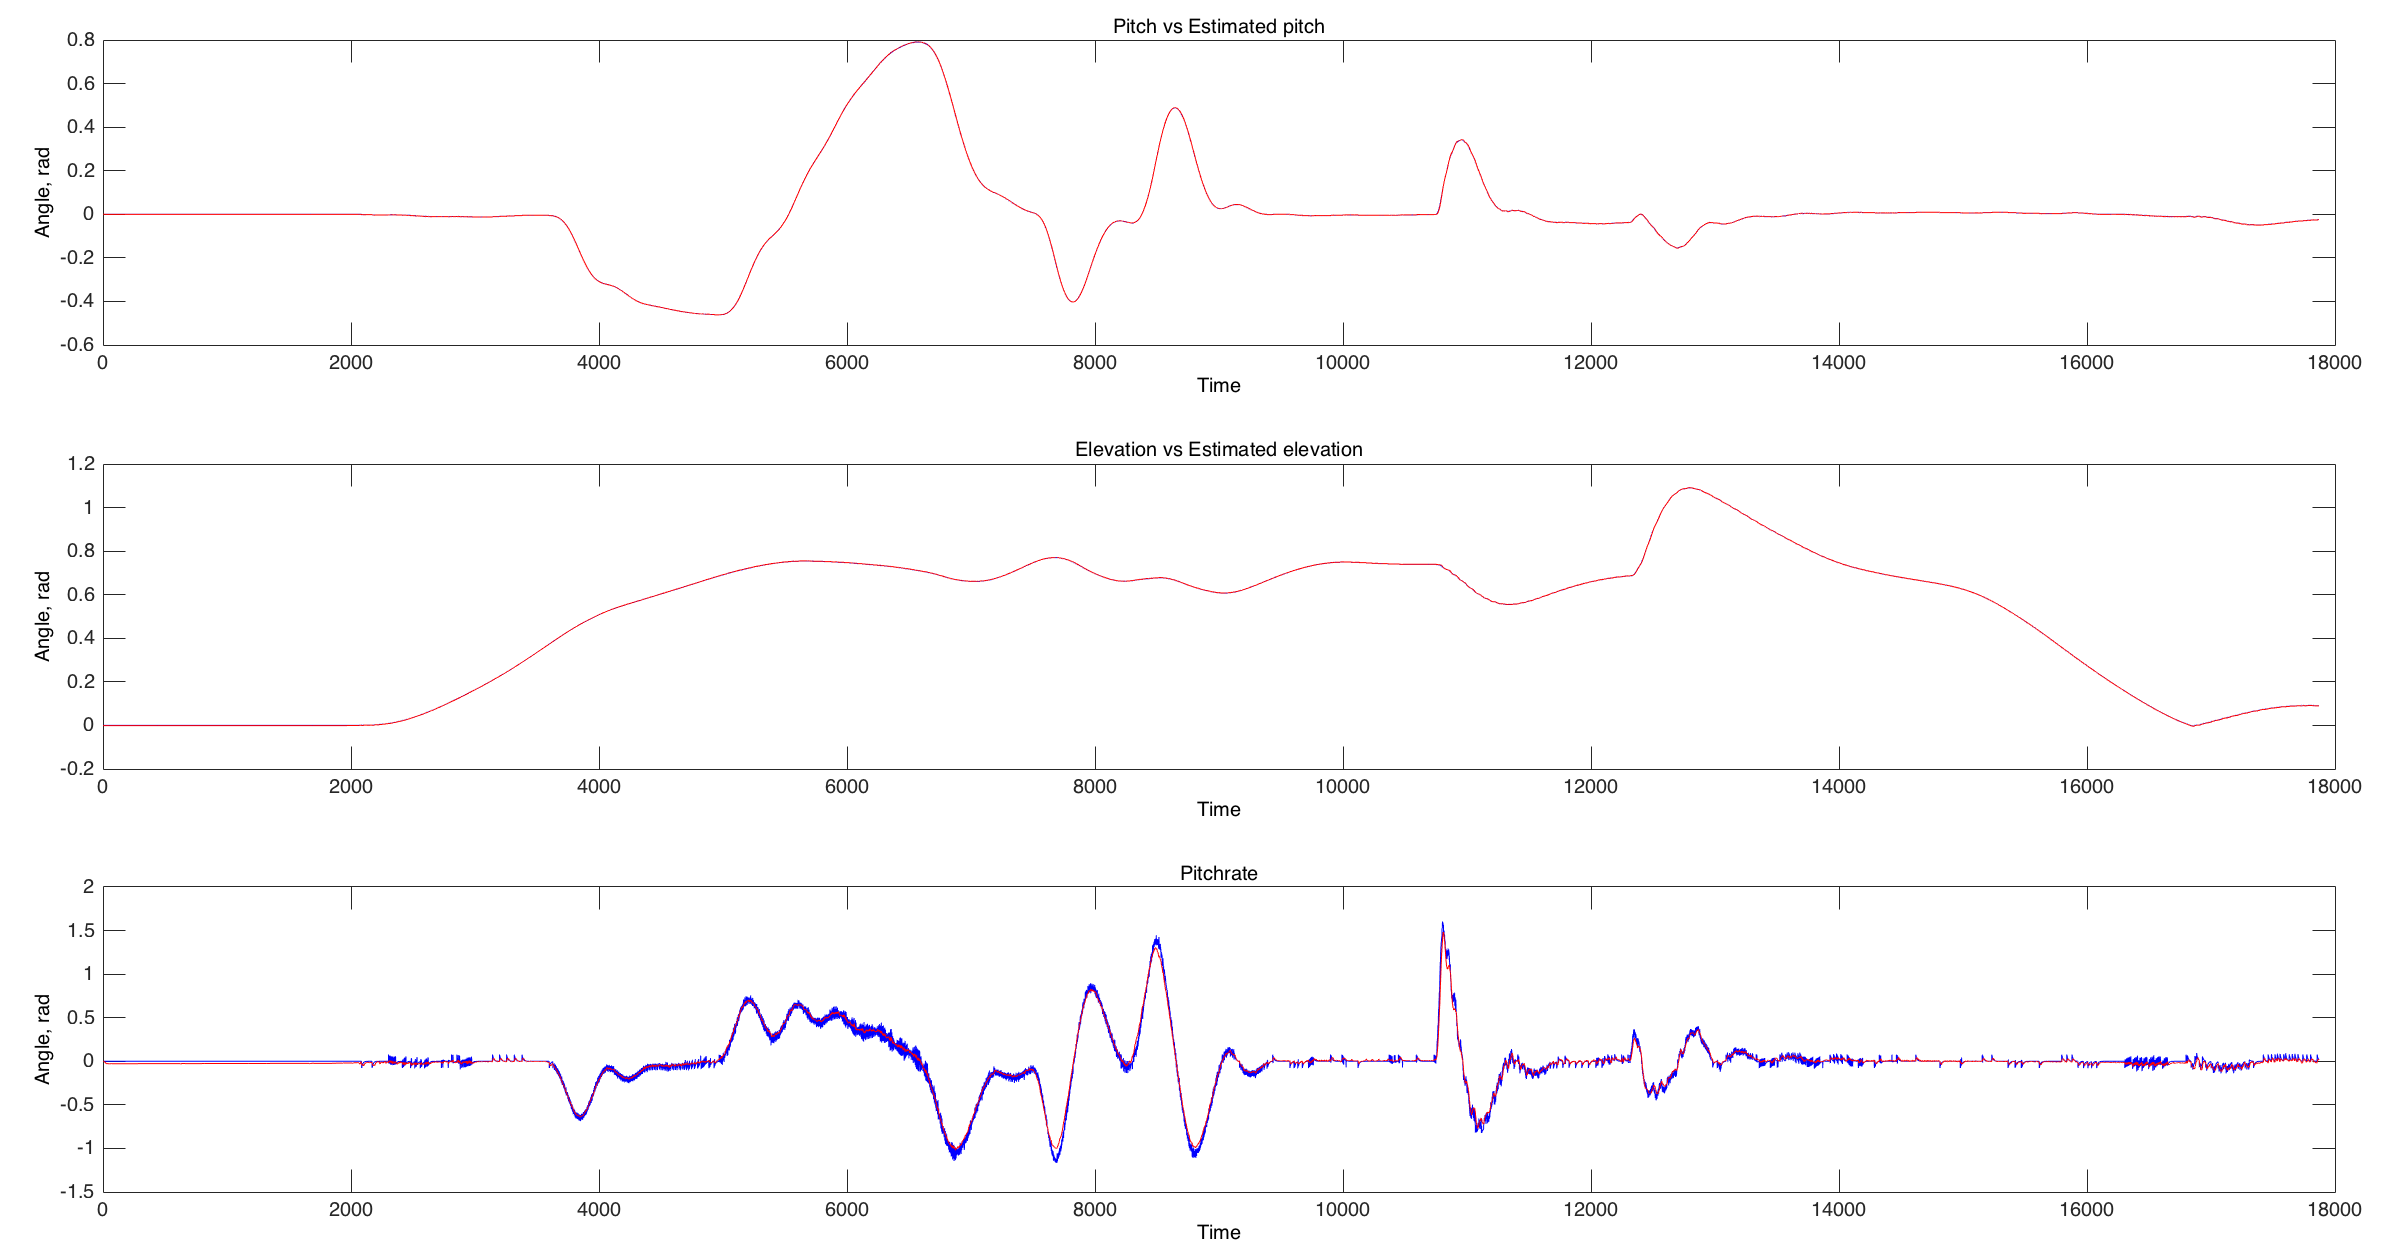
\includegraphics[width=1.0\textwidth]{pitchrate_PI.png}
    \caption{Comparison of measured and estimated values of pitch, elevation and pitch rate in the PI-controller (\emph{\color{blue}Blue} = measured value, \emph{\color{red} red} = estimated value)}
    \label{fig:plot3}
\end{figure}

\begin{figure}[H]
    \centering
    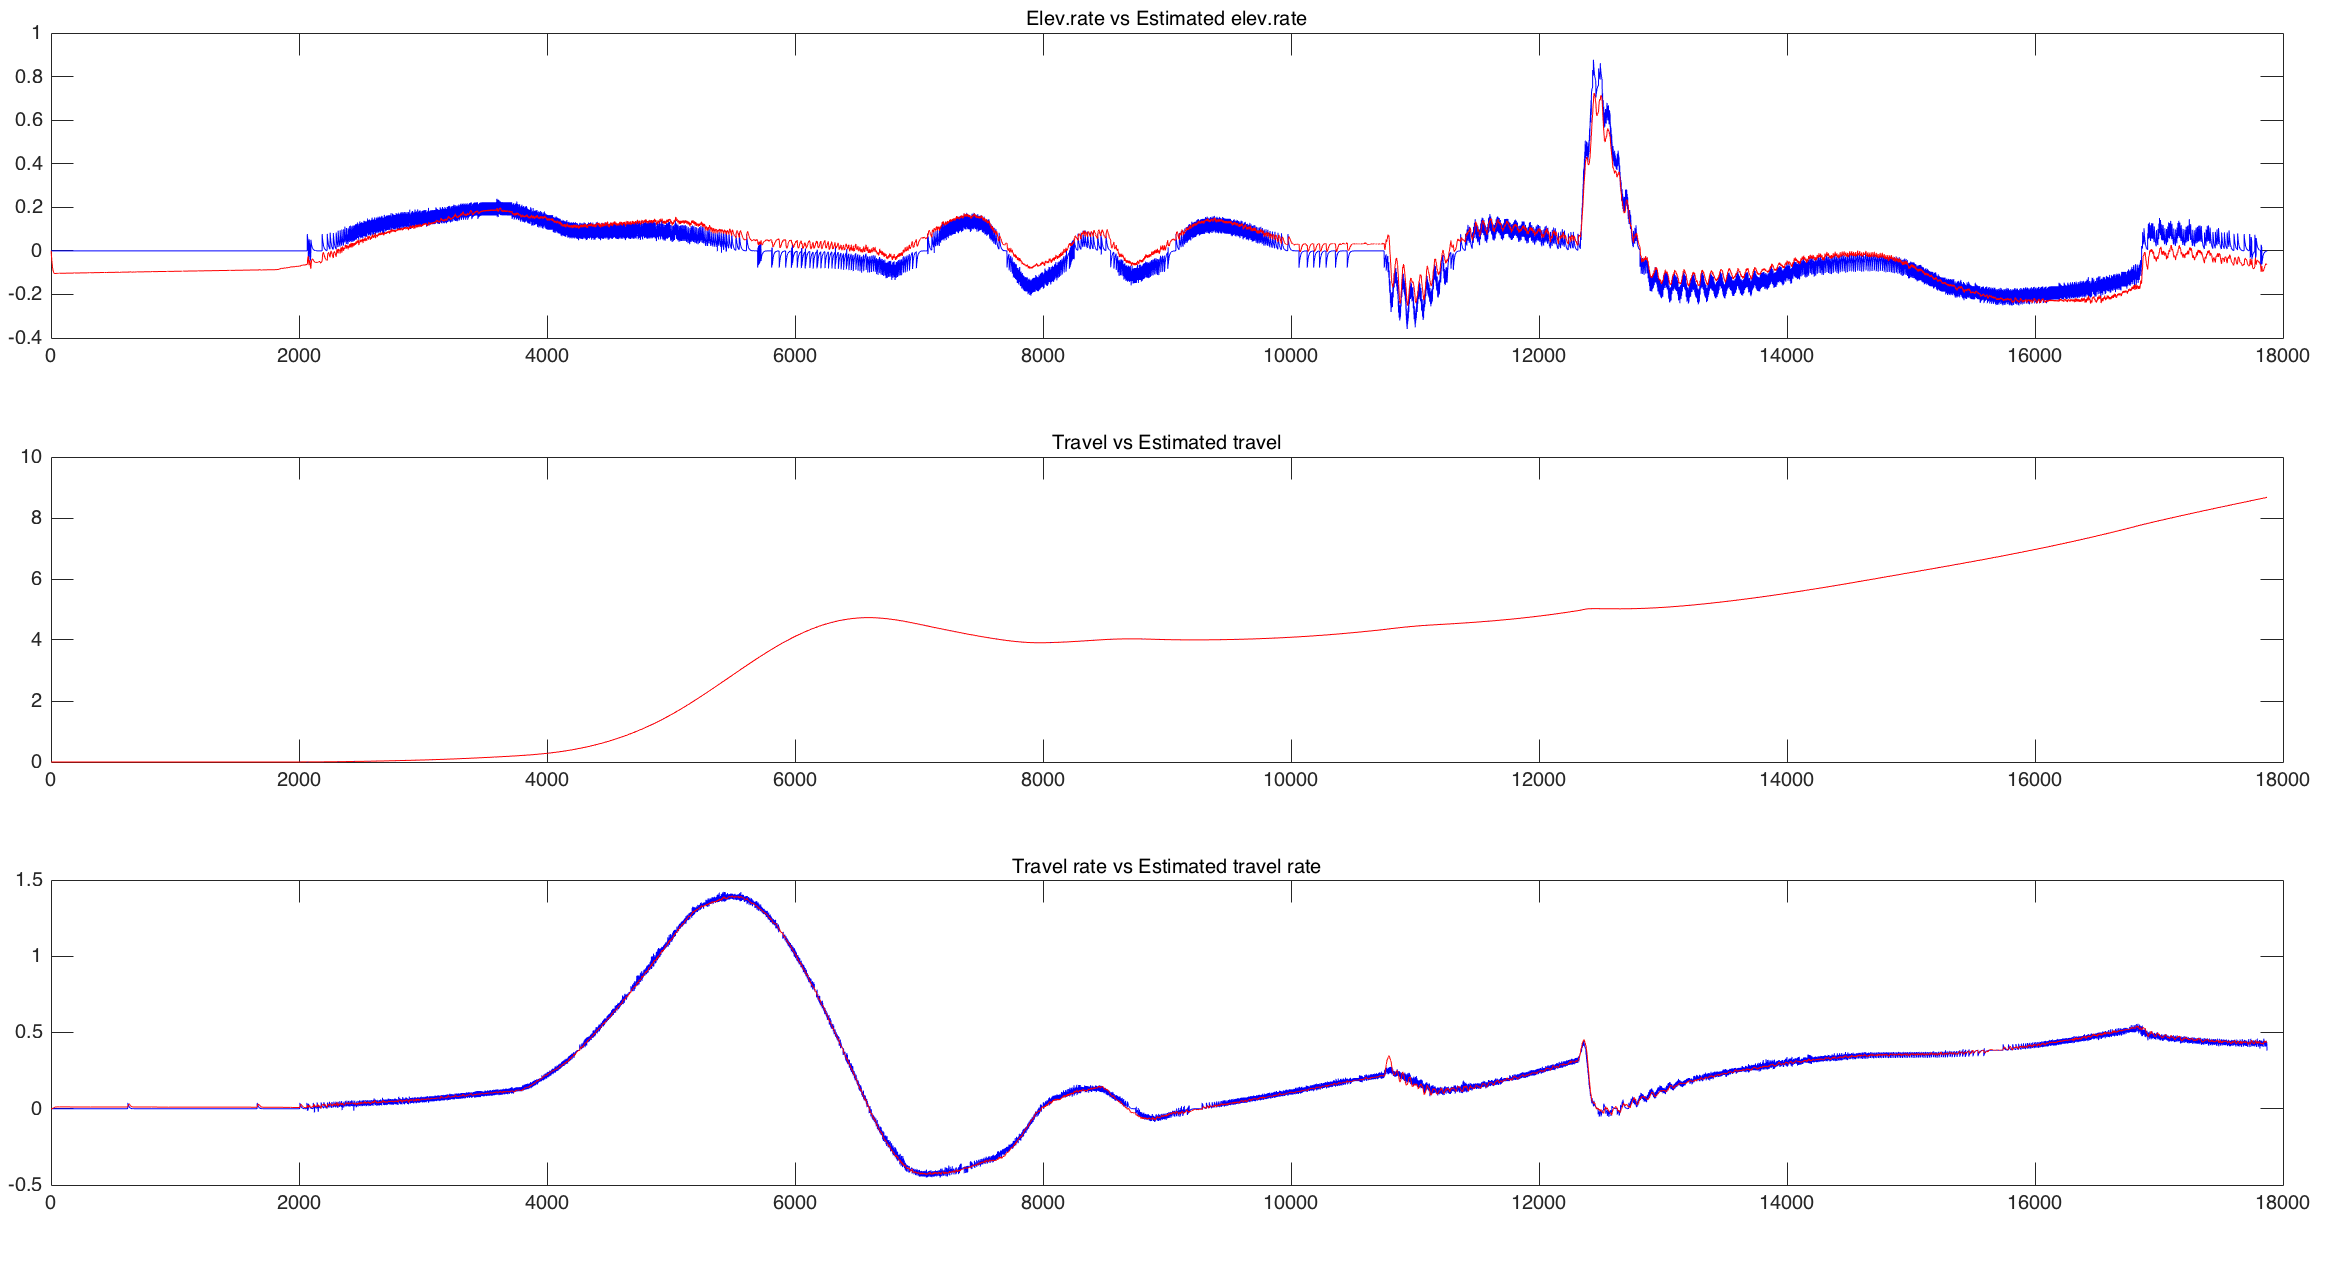
\includegraphics[width=1.0\textwidth]{elevrate_PI.png}
    \caption{Comparison of measured and estimated values of elevation rate, travel and travel rate in the PI-controller (\emph{\color{blue}Blue} = measured value, \emph{\color{red} red} = estimated value)}
    \label{fig:plot4}
\end{figure}

%
\begin{figure}[H]
    \centering
    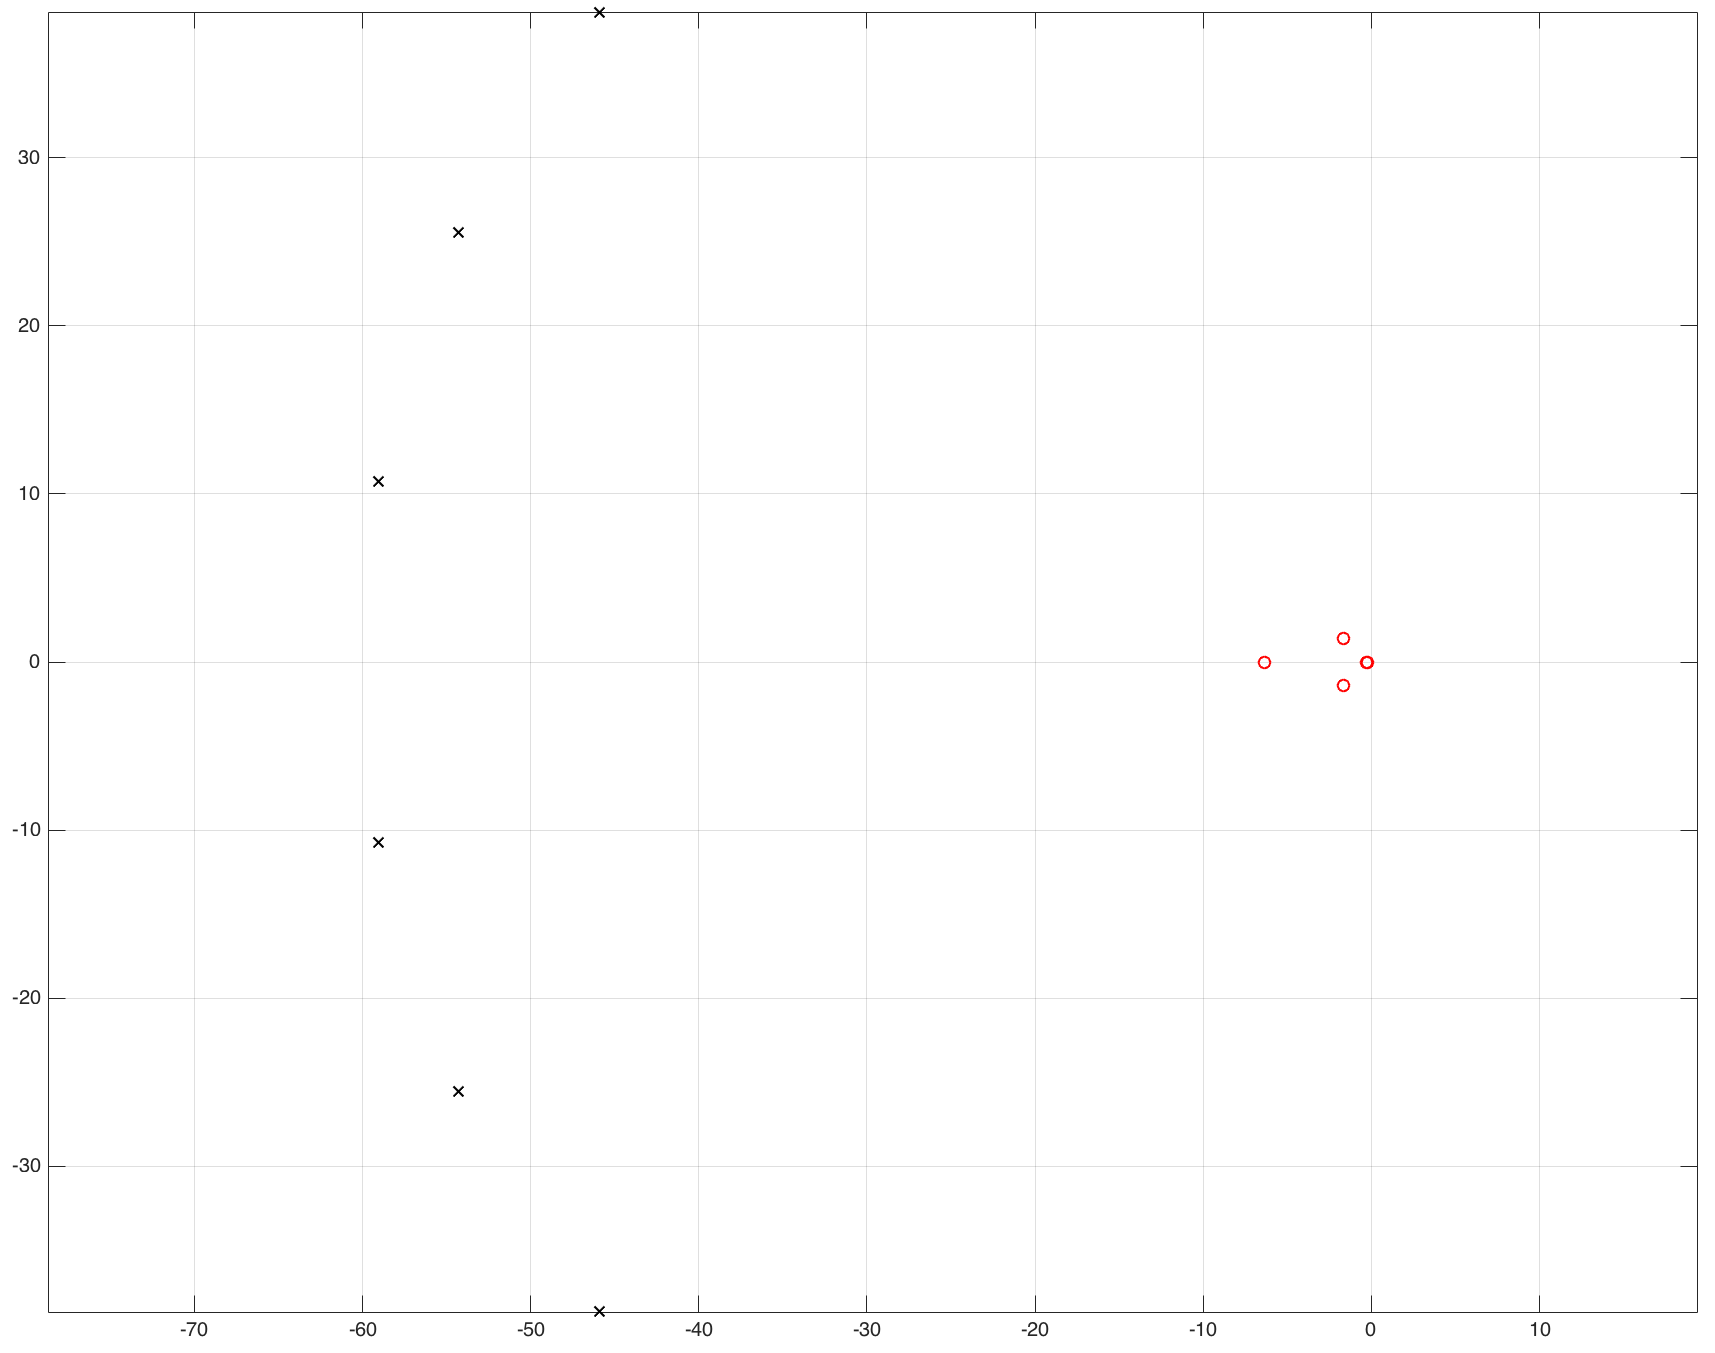
\includegraphics[width=\textwidth]{poleplacement.png}
    \caption{Pole plot of the chosen pole placements (black) and the systems eigenvalues (\emph{\color{red} red}).}
    \label{fig:poles}
\end{figure}
%

\subsection{Observer Using $\tilde{e}$ and $\tilde{\lambda}$}

With the measurable states given in the lab assignment, we alter the output matrices and get the following observability matrices
$$ 
\mathcal{O}_{\tilde{e}\tilde{\lambda}} = 
        \fixTABwidth{T}
        \bracketMatrixstack{
            0&0&1&0&0&0\\
            0&0&0&0&1&0\\
            0&0&0&1&0&0\\
            0&0&0&0&0&1\\
            0&0&0&0&0&0\\
            K_3&0&0&0&0&0\\
            0&0&0&0&0&0\\
            0&K_3&0&0&0&0\\
            0&0&0&0&0&0\\
            0&0&0&0&0&0\\
            0&0&0&0&0&0\\
            0&0&0&0&0&0
        }
    \quad
\mathcal{O}_{\tilde{p}\tilde{\lambda}} = 
        \fixTABwidth{T}
        \bracketMatrixstack{
            1&0&0&0&0&0\\
            0&0&0&0&1&0\\
            0&1&0&0&0&0\\
            0&0&0&0&0&1\\
            0&0&0&0&0&0\\
            K_3&0&0&0&0&0\\
            0&0&0&0&0&0\\
            0&K_3&0&0&0&0\\
            0&0&0&0&0&0\\
            0&0&0&0&0&0\\
            0&0&0&0&0&0\\
            0&0&0&0&0&0
        }
$$
with  $\text{rank}(\mathcal{O}_{\tilde{e}\tilde{\lambda}}) = 6$ and $\text{rank}(\mathcal{O}_{\tilde{p}\tilde{\lambda}}) = 4$. Thus the system is unobservable for 
$\vec{y} = [\tilde{p} \enskip \tilde{e}]^T$, but observable for $\vec{y} = [\tilde{e} \enskip \tilde{\lambda}]^T$. \\

Using $\vec{y} = [\tilde{e} \enskip \tilde{\lambda}]^T$ as the basis for the linear observer gave, using similar controller tuning as previously, very poor performance, especially in controlling the pitch (see \cref{fig:crazyplot1}, \cref{fig:crazyplot2}). This makes sense, as we then are trying to control the helicopter pitch using only the elevation- and travel angles, which is no straight forward task. The controllability matrix suggests it is possible, as the travel is given by the pitch (\ref{eq:6c}), but it requires extensive tuning.
\
%
\begin{figure}[H]
    \centering
    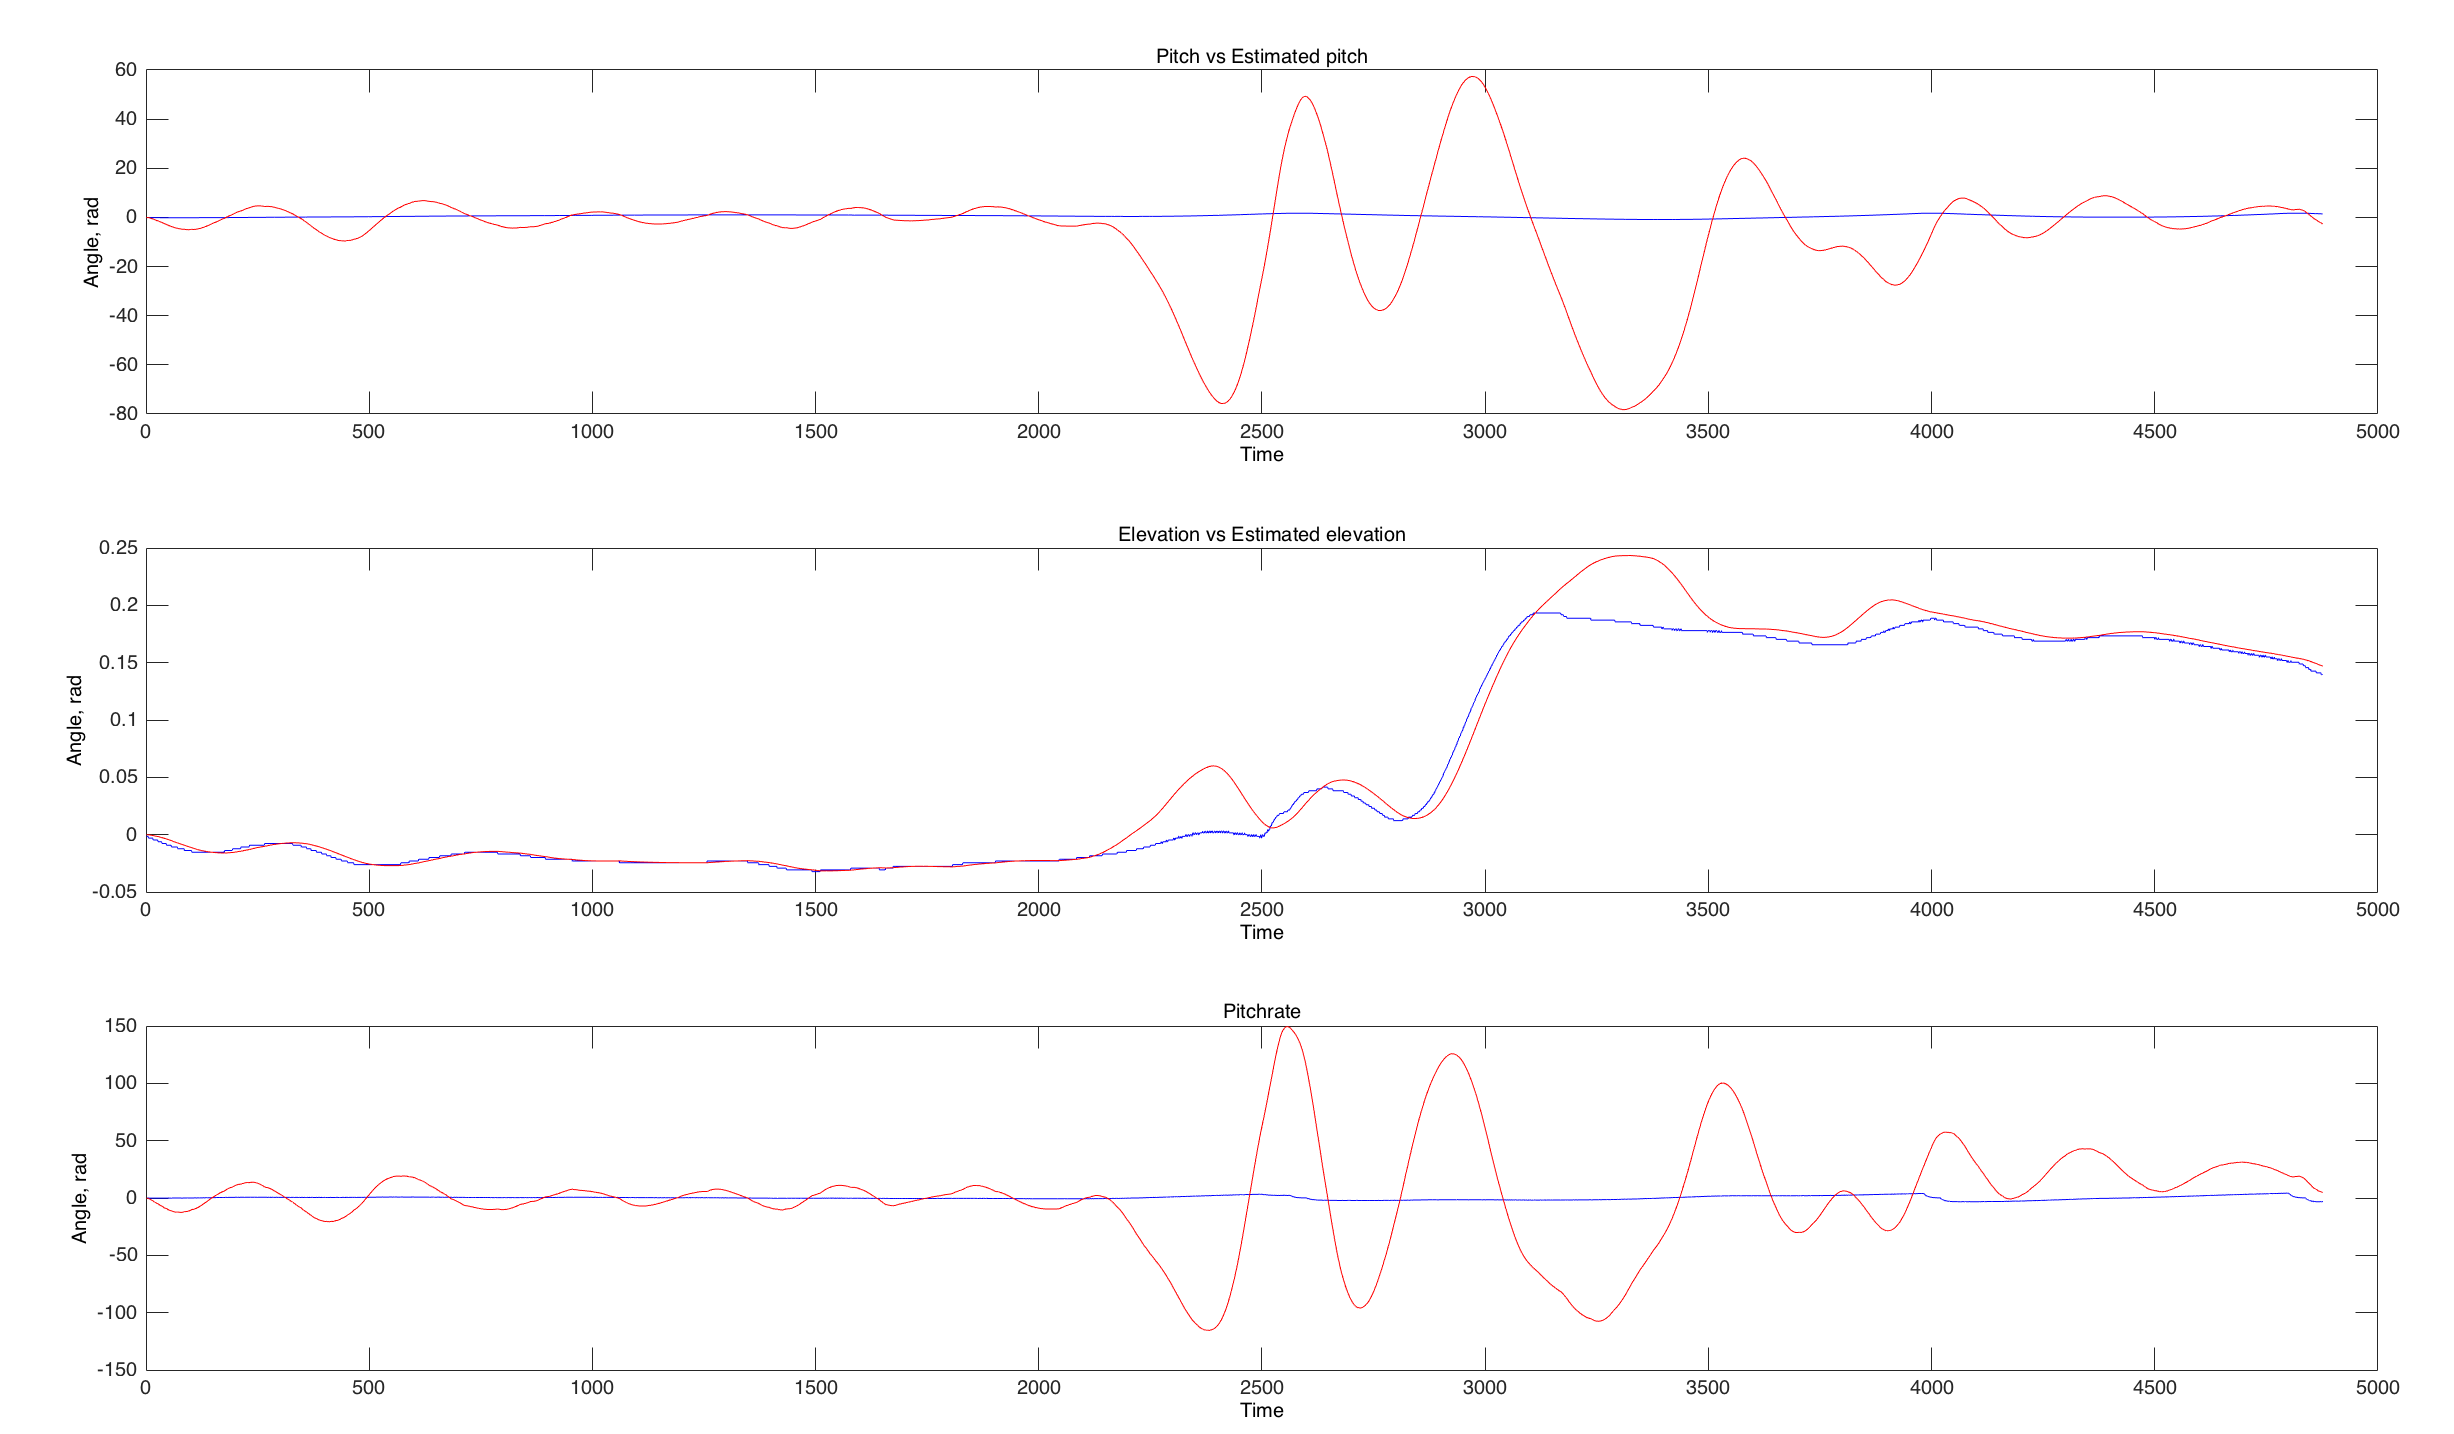
\includegraphics[max size={\textwidth}{\textheight}]{crazyplot2.png}
    \caption{Plot of the true (\emph{\color{blue} blue}) and observed (\emph{\color{red} red}) values of the pitch, elevation and elevation rate.}
    \label{fig:crazyplot1}
\end{figure}
%
\begin{figure}[H]
    \centering
    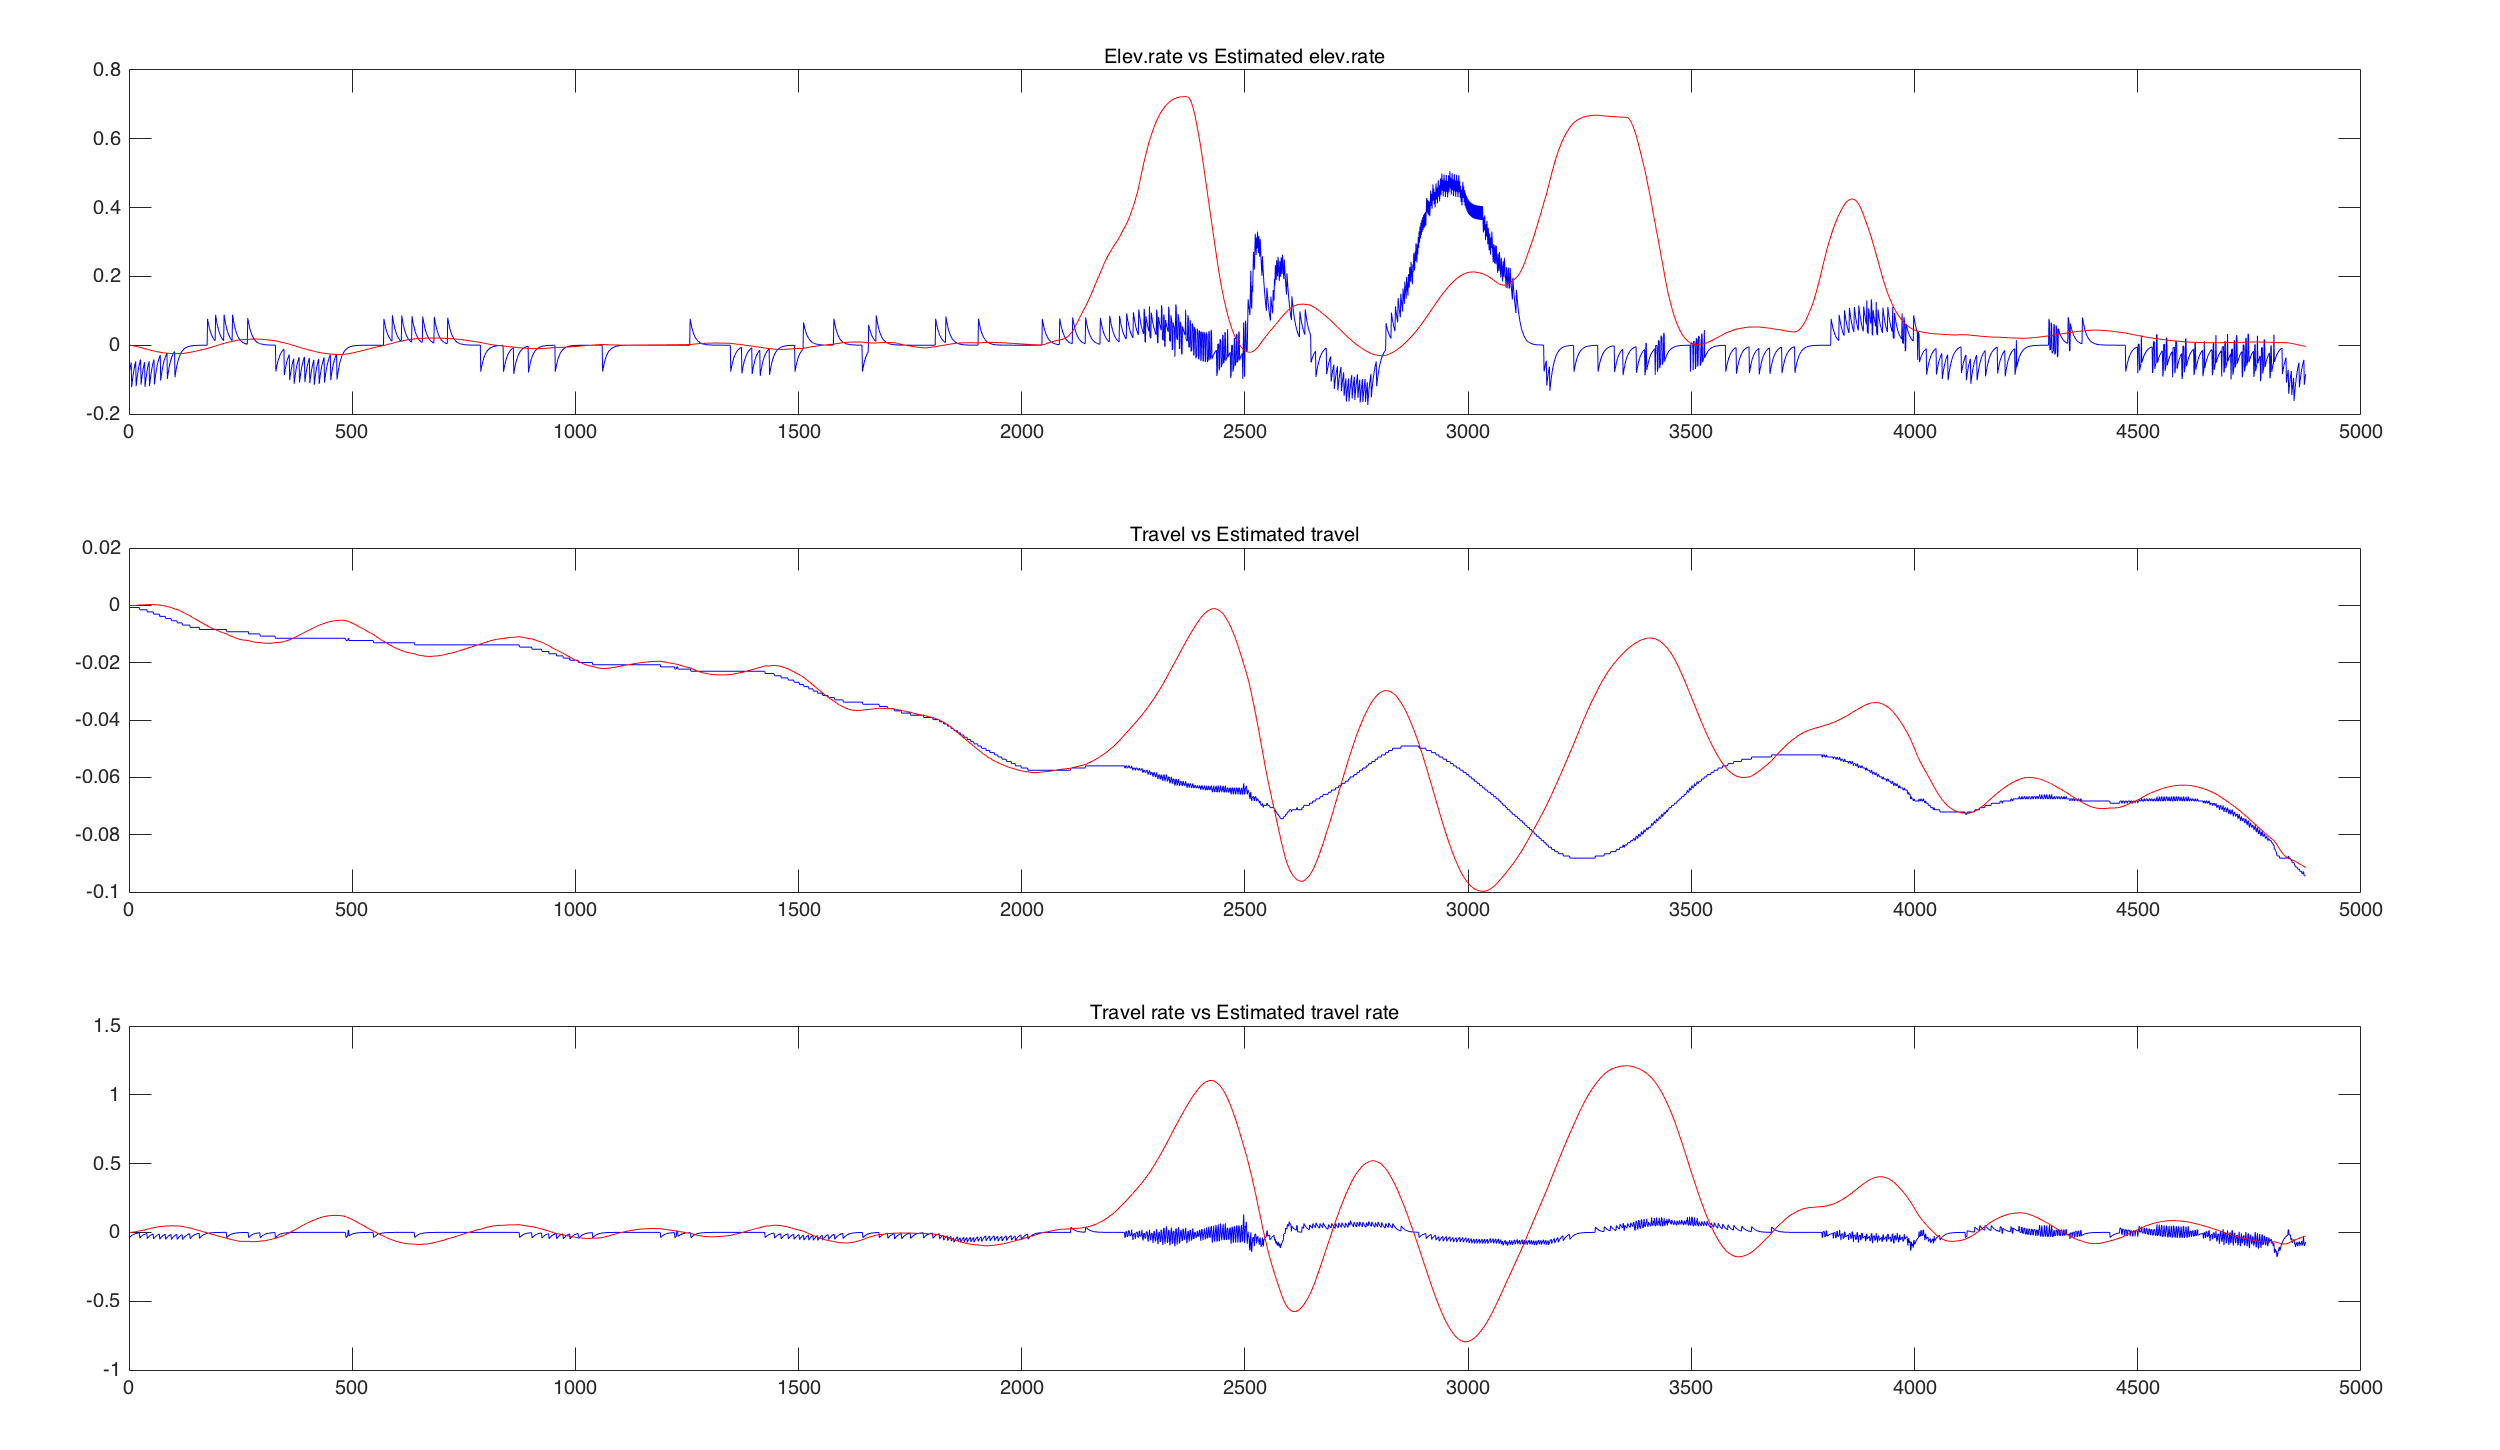
\includegraphics[max size={\textwidth}{\textheight}]{crazyplot1.png}
    \caption{Plot of the true (\emph{\color{blue} blue}) and observed (\emph{\color{red} red}) values of the elevation rate, travel, and travel rate.}
    \label{fig:crazyplot2}
\end{figure}
%
%\input{summary}

\newpage 
%\addcontentsline{toc}{section}{References} %uncomment if you want the references included in the table of content
\bibliographystyle{ieeetr}
\bibliography{ref.bib}






\end{document}
